\graphicspath{{chapters/ThebasicsImages/}}


\chapter{Introduction}

\textbf{\textit{Written by Chiara Campanelli}}

\section{Basic principles} \label{chap: Basics}

\begin{figure}[H]
  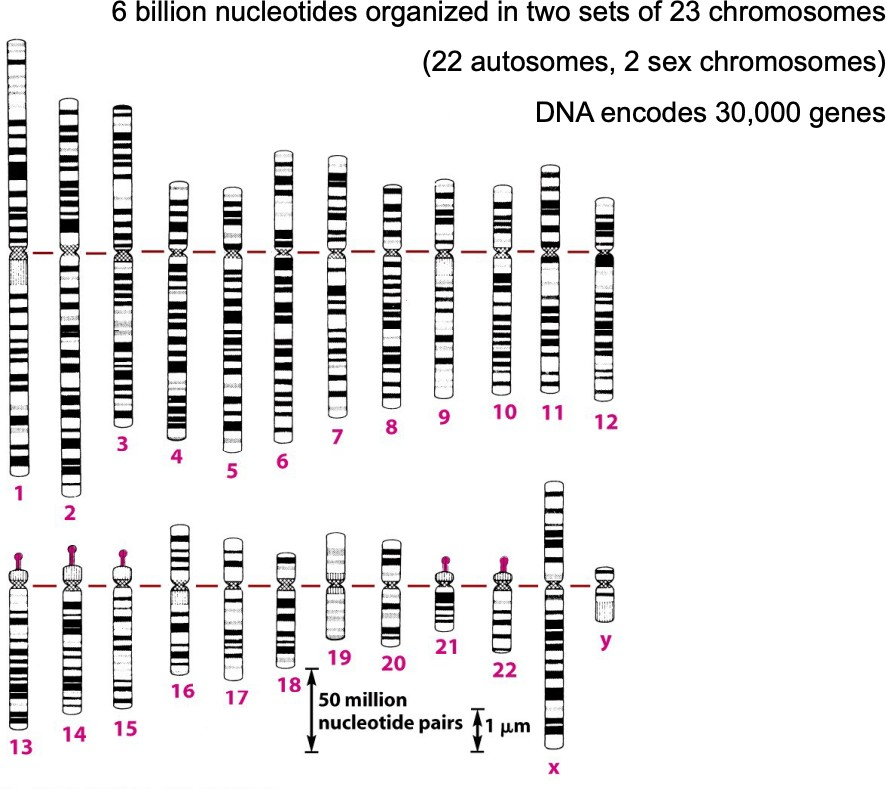
\includegraphics[width=4.32507in,height=3.86281in]{image1.jpeg}
  \centering
  \caption{}
\end{figure}


The words variations, aberrations and lesions are often interchanged.
Aberrations and lesions are mainly used for acquired lesions, instead variations
are mainly used for the inherited ones.

\hypertarget{genetic-make-up}{%
\subsection{Genetic Make-Up}\label{genetic-make-up}}

\begin{figure}[H]
  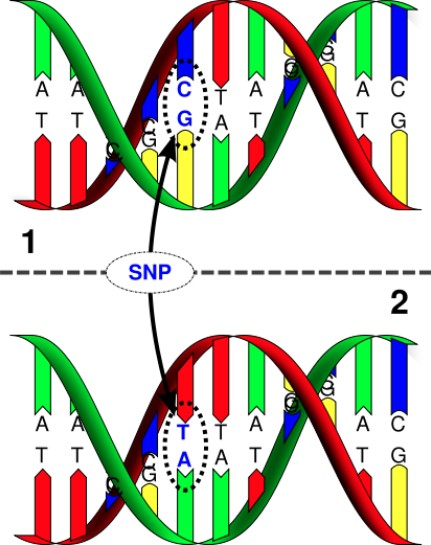
\includegraphics[width=1.97816in,height=2.50248in]{image2.jpeg}
  \centering
  \caption{}
  \label{fig: SNP}
\end{figure}


\textbf{Single Nucleotide Polymorphism} (SNP) is a sequence variation affecting
single bases (point mutations) (figure \ref{fig: SNP}).

The genomes of two unrelated individuals have about 1\% of different bases →
that percentage corresponds to the SNPs.

But looking at the \textbf{Copy Number Variants} (CNV), that difference will be
way higher than only 1\% DNA not present in only two copies, but in multiple,
single or even zero copies (hemizygous loss, homozygous loss). They are less
known as inherited type of variants because they are harder to detect and
identify, but they provide a lot of uniqueness in each of us.


\begin{figure}[H]
  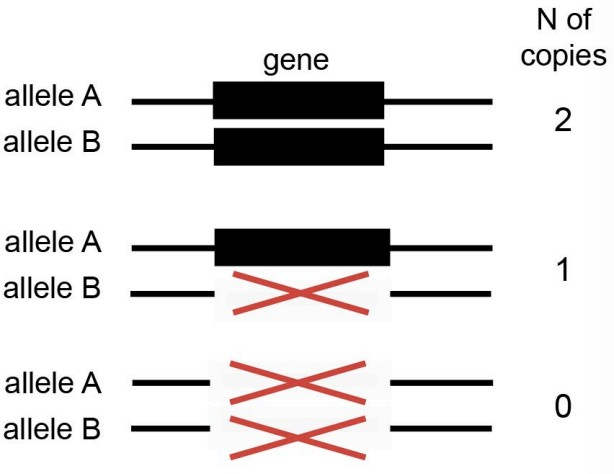
\includegraphics[width=2.93475in,height=2.26167in]{image3.jpeg} 
  \centering
  \caption{}
  \label{fig: SNP2}
\end{figure}


Why are SNPs and CNVs so important?

They are responsible of human diversity → genetic changes

Hundreds of CNVs per individual and 20\% of them potentially affect protein-
coding genes

\textbf{Differences} in Genetic Make-up:

Very common variants are variants that are distributed in the population as the
common allele, so that 1/2 of the population has an heterozygous genotype at
that position, 1/4 has an homozygous genotype for one allele and 1/4 has an
homozygous genotype for the other allele.

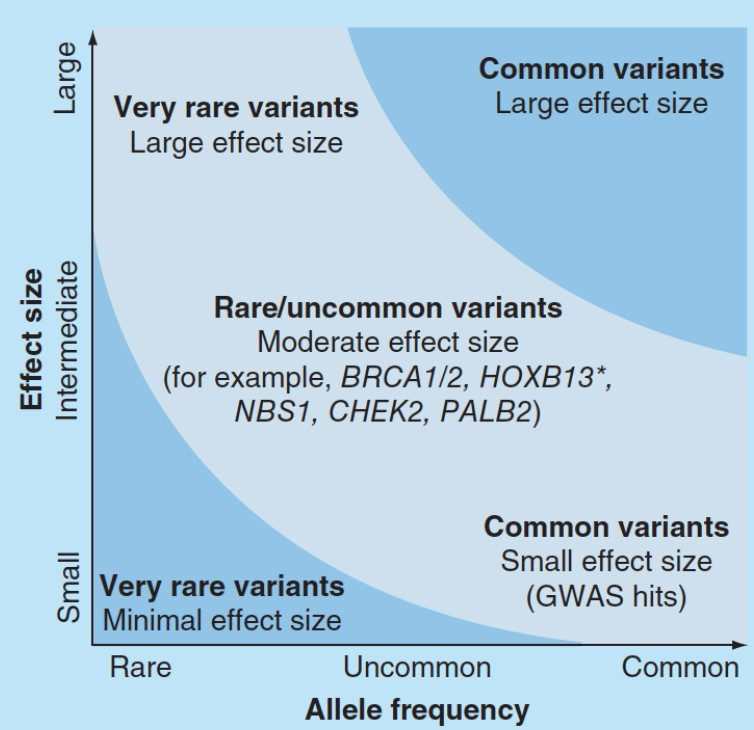
\includegraphics[width=3.9928in,height=3.87812in]{image4.jpeg}

The \textbf{penetrance} is the proportion of individuals carrying an allele (or
a genotype) that also expresses the trait (phenotype) associated with it.
Obviously, penetrance is directly associated with the size of the effect
produced by the variant.

The \textbf{allele frequency} is calculated by dividing the number of times the
allele of interest is observed in a population by the total number of copies of
all the alleles at that particular genetic locus in the population.

The allele frequency is low with very rare variants

Well known variants: BRCA1/2, HOXB13, NBS1, PALB2, CHEK2 → they have moderate
size effects, meaning that all the people who have the variants, have the
disease


\hypertarget{differences-in-genetic-make-up-example}{%
\subsubsection{Differences in genetic Make-Up,
example}\label{differences-in-genetic-make-up-example}}
% article to be read? #TODO


Absorption, distribution, metabolism and elimination (ADME) genetic variants
determine pharmacokinetic variability of certain compounds, influencing the
patients' treatment response. Both common and rare variants are involved.

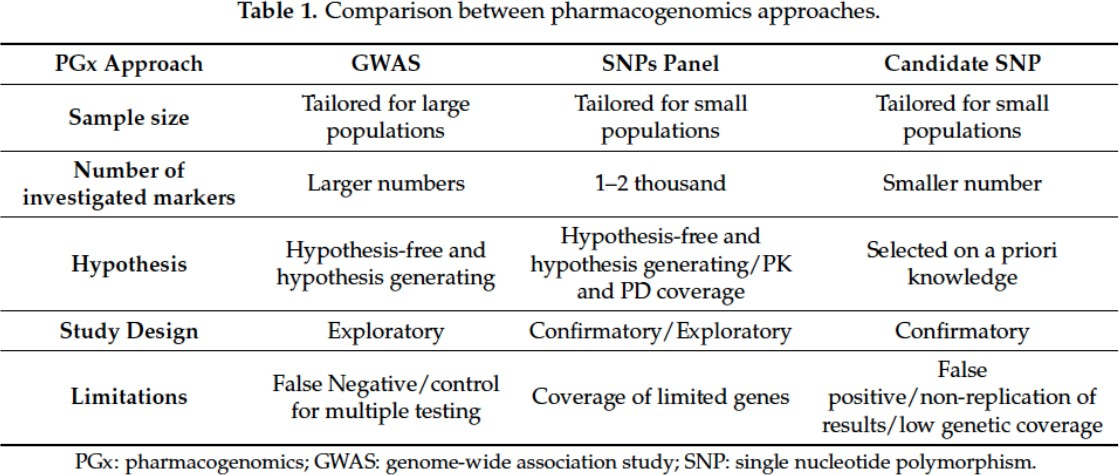
\includegraphics[width=6.18852in,height=2.6224in]{image5.jpeg}

Three main ways to study genetic variants: 

\begin{itemize}
  \item GWAS (genome-wide association study)
  \item SNPs panel
  \item Candidate SNP
\end{itemize}




For example, in terms of hypothesis, if I study all the variants in the human
genome and I query them in a large population, I generate data without
specifying SNP to search. Instead, if I have a very specific hypothesis, for
example I want to query if a SNPs in the CYP gene relates to the conversion of
androgens to estrogens, I don't need to run an GWAS or a wide SNPs panel. I can
query those SNPs because I have an \emph{a priori} hypothesis and I want to test
them.

This type of differential design for an experiment it is not only true for
inherited variants and ADME genes, but also to predisposition to diseases and to
study human tumors.

Precision medicine → treatment (or dosage) of a patient based on their
individual traits: takes into consideration genetic and genomic of the
individual and tumor/disease cells

\begin{itemize}
  \item Drink beer and turn red → ADME gene
  \item Athletes with a deletion of a gene, the steroids were not found in the
  anti-doping tests
\end{itemize}
 

\hypertarget{acquired-dna-aberrations}{%
\subsection{Acquired DNA aberrations}\label{acquired-dna-aberrations}}


Somatic variants are the variants NOT inherited from parents and not transmitted
to offspring. They are:

\begin{itemize}
  \item \textbf{Single Nucleotide Variants} (SNV) are somatic changes of single
  nucleotides present in only certain cells, instead of SNPs that are present in
  all cells of our body.
  \item \textbf{Indels} are changes that involve few nucleotides by INsertion
  and DEletion
  \item \textbf{Rearrangements} are mutations that can involve events like
translocations, inversion, chromothripsis,.. usually these events are caused by
breakage in the DNA double helices a two different locations, followed by a
rejoining of the broken ends to produce a new chromosomal arrangement of genes,
different from the beginning

  \item \textbf{Somatic copy number aberrations} (\textbf{SCNA}) are somatic
changes similar to CNVs. They can be every change related to the number of
copies like loss of a portion of a genome, loss of both alleles, extra copies...
\end{itemize}

\begin{figure}[H]
  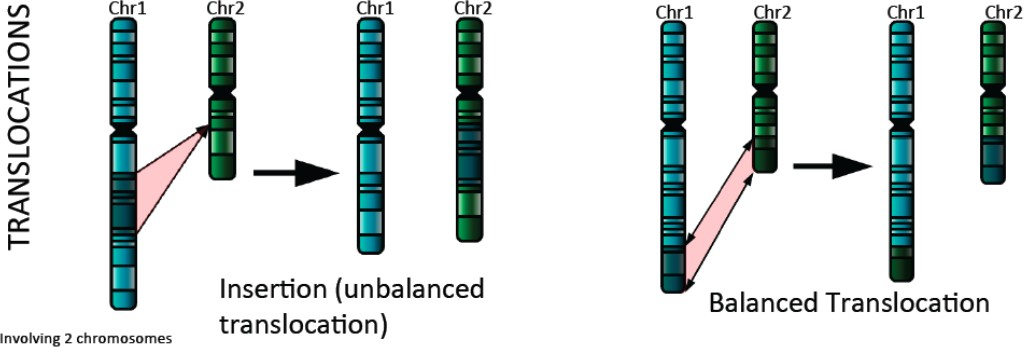
\includegraphics[width=6.1748in,height=2.09646in]{image6.jpeg}\\
  \centering
  \caption{translocations}
  \label{fig: translocations}
\end{figure}

Rearrangements include:

\begin{itemize}
  \item \textbf{Balanced translocation} (figure \ref{fig: translocations}): you conserve the quantity of DNA, there
  isn't any loss or gain.
  
  \item \textbf{Unbalanced translocation}: A genomic portion is translocated
  from a chromosome to another, there is not vice versa.
  
  \item \textbf{Inversions} in only ONE chromosome: everything is normal instead
  in the break points.

  \begin{figure}[H]
    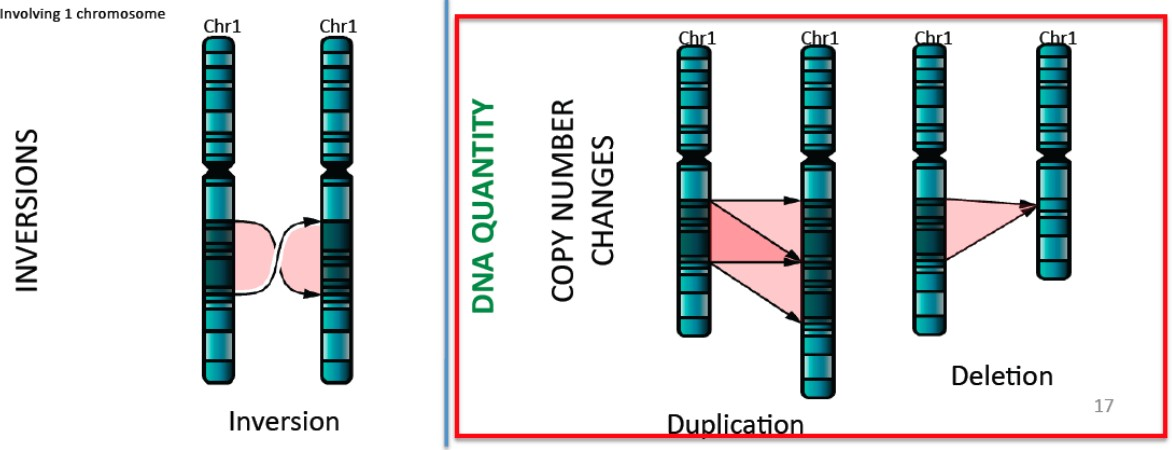
\includegraphics[width=6.22722in,height=2.39062in]{image7.jpeg}
    \centering
    \caption{Duplications inversions and deletions}
    \label{fig: Duplications inversions and deletions}
  \end{figure}

  \item \textbf{Copy number changes:} duplication or deletion. It could happen in
  the same chromosome but also in different chromosomes.
\end{itemize}

Other important modifications:

\begin{itemize}
  \item \textbf{Chromoplexy}: a class of complex somatic DNA rearrangements
  whereby abundant DNA deletions and intra- and inter-chromosomal translocations
  that have originated in an interdependent way occur within a single cell
  cycle.

  \item \textbf{Chromothripsis}: a clustered chromosomal rearrangement in
  confined genomic regions that results from a single catastrophic event,
  usually limited to one chromosome.

  \item \textbf{Kataegis}: a phenomenon that is characterized by large cluster
  of mutations (hypermutation) in the genome of cancer cells. An APOBEC family
  enzyme might be responsible fo the kataegis process.
\end{itemize}
  
\begin{figure}[H]
  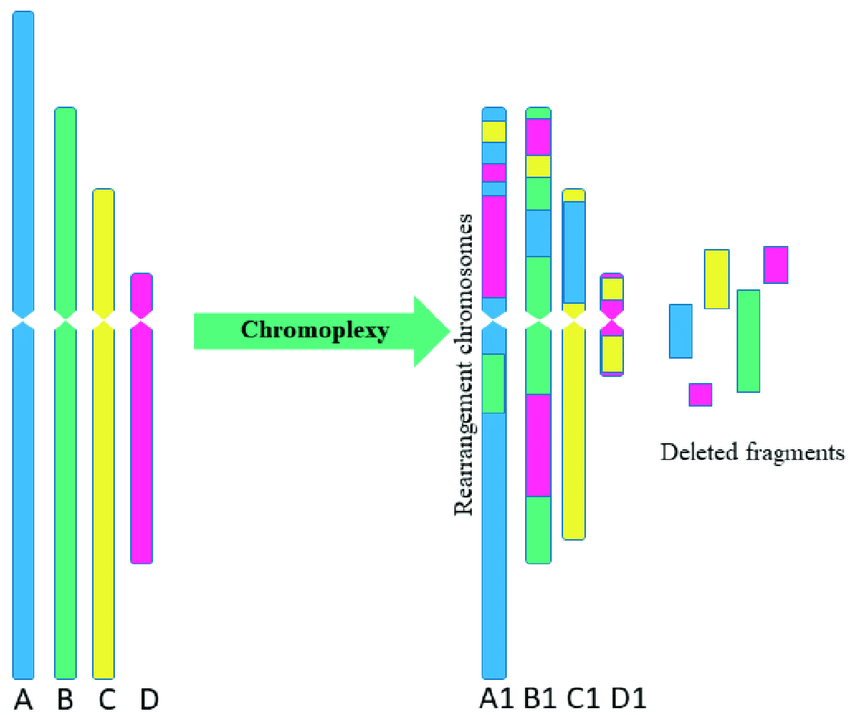
\includegraphics[width=3.81944in,height=3.21433in]{image8.png}\\
  \centering
  \caption{Chromoplexy}
  \label{fig: Chromoplexy}
\end{figure}


When an aberration (clonal) occurs, all the cells will harbour the aberration
and at some point another aberration (subclonal of the other) could appear in
just one cell line. The \textbf{clonal} aberration is present in all the cells,
the \textbf{subclonal} aberration is inherited in just one cell line. Clonality
is an important information that allow us to study evolution.


\hypertarget{experimental-approaches}{%
\section{Experimental approaches}\label{experimental-approaches}}


Experimental techniques to detect variants/aberrations \textbf{prior to NGS}: a
failure because it was very hard to determine the starting points of the
aberrations. %#TODO which tecniques? 

\begin{figure}[H]
  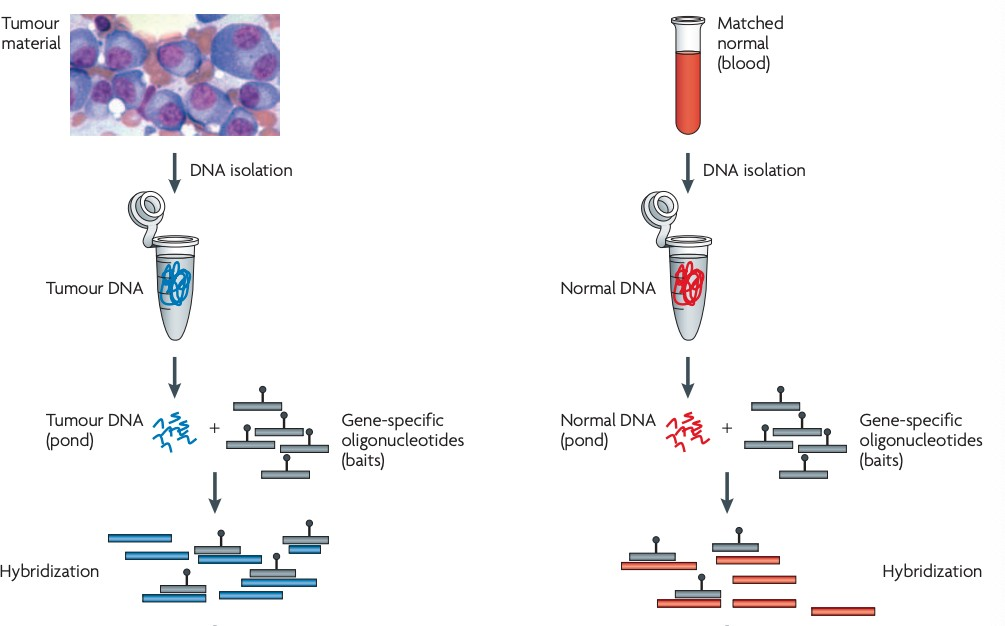
\includegraphics[width=6.18343in,height=3.84729in]{image9.jpeg}
  \centering
  \caption{Meyerson et al. 2010, ``Advances in Understanding Cancer Genomes
  through Second-Generation Sequencing.'', Nature Reviews Genetics,
  \url{https://doi.org/10.1038/nrg2841}}
  \label{fig: DNA variants}
\end{figure}

Bulk of tumor tissue/cells from the blood procedure (figure \ref{fig: DNA variants}):


\begin{enumerate}
\def\labelenumi{\arabic{enumi})}
\item
  DNA isolation.
\item
  Gene-specific oligonucleotides (\textbf{baits}) that get hybridized onto the
  tumor DNA → the baits have a tag that allows them to be isolated.
\item
  The DNA does get fragmented.
\item
  The captured DNA is eluted and prepared into sequencing libraries.
\item
  Sequencing.
\item
  Aligned to the bait sequences.
\end{enumerate}


We repeat the procedure for healthy cells of the same individual in order to
\textbf{detect somatic mutations}.

\begin{figure}[H]
  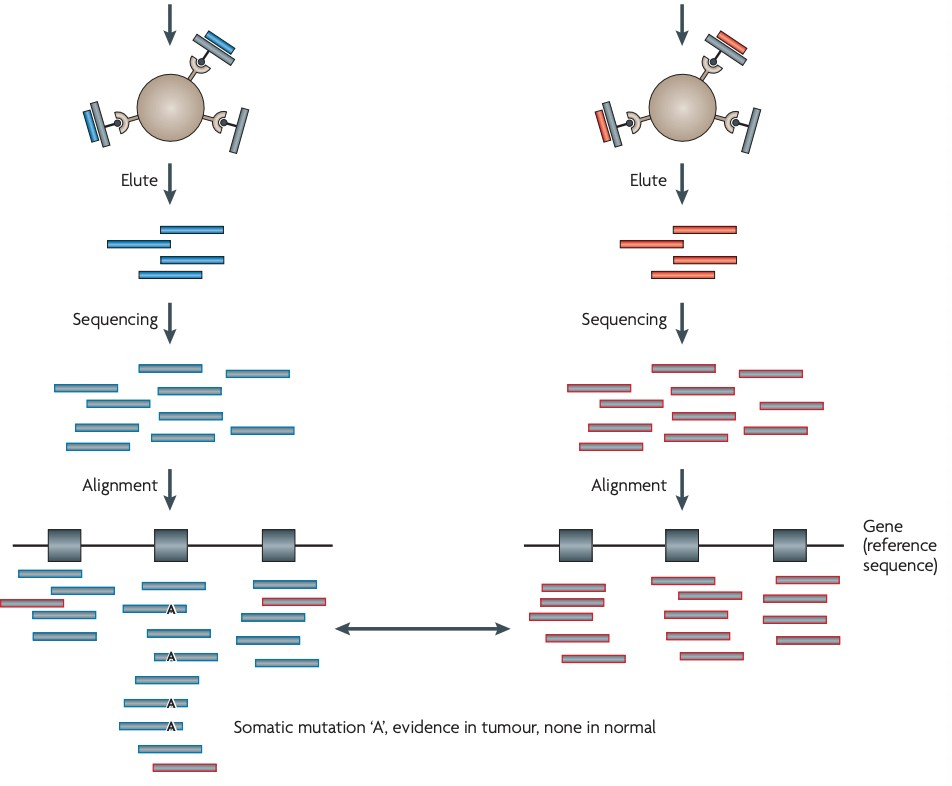
\includegraphics[width=6.14828in,height=5.07625in]{image10.jpeg} \label{fig:
  DNA cancer variants detection}
  \centering
  \caption{Beads capture}
\end{figure}


We sequence baits because is way cheaper (exons of 50 bases instead the whole
genome)

After fragmentation procedure, before adding the adapters, we can choose between
two different sequencing approaches \ref{fig: sequencing methods}:\\


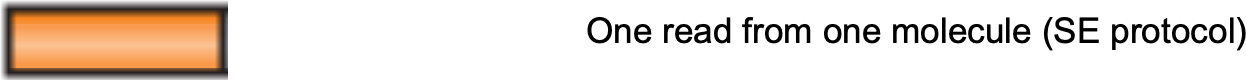
\includegraphics[width=0.75\textwidth]{image11.png}\\ \label{fig: sequencing
methods}
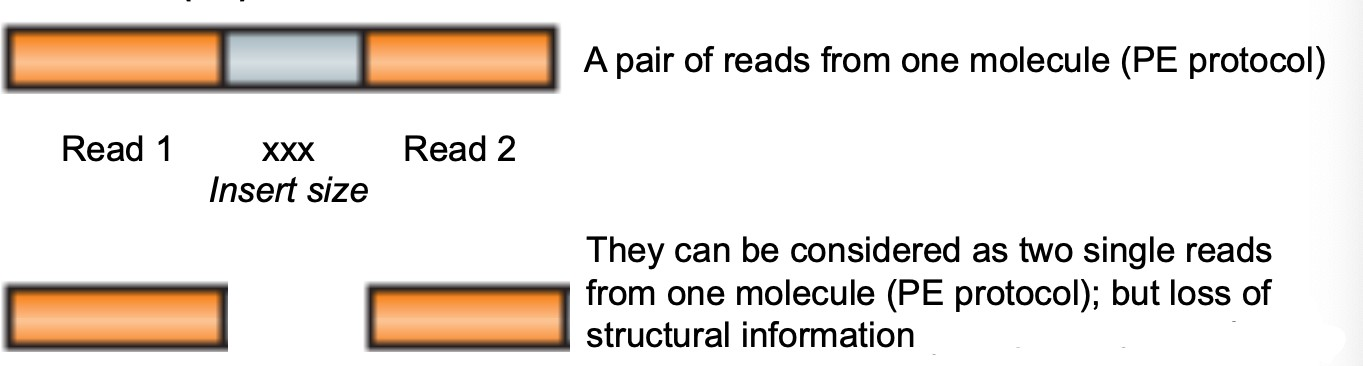
\includegraphics[width=0.75\textwidth]{image12.jpeg}

\begin{itemize}
  \item \textit{\textbf{Paired End (PE) sequencing}}

  You will sequence only one part of a molecule (length of 150 bp → based on the
  power of the sequencing machine we are using). You will know exactly 150 bp
  for every molecule you sequence, but you lose information (the second end of
  the pair).

  \item \textit{\textbf{Single End (SE) sequencing}}
  
  You information about the length of the DNA portion between the ends. It's
  more expensive, but:

  \begin{itemize}
    \item
      it gives information about the localization of the molecule
    \item
      you can treat each end as single read
    \end{itemize}

\end{itemize}


\subsection{Information after reads mapping over reference genome}

\begin{figure}[H]
  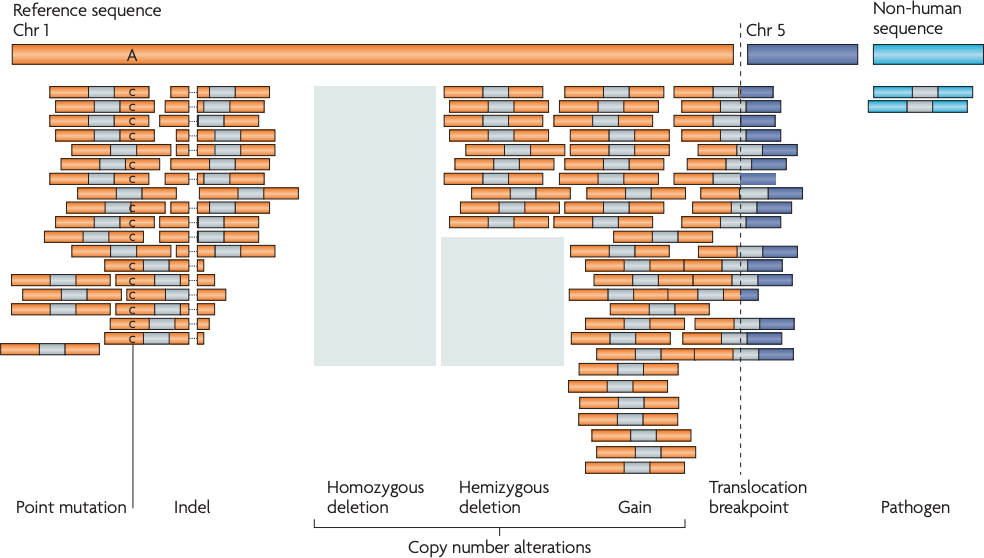
\includegraphics[width=6.16003in,height=3.4875in]{image13.png}
  \centering
  \caption{In the following picture: a view of reads that are mapped against
  reference genome and what we would look if we have any of the variations that
  we mentioned}
\end{figure}

Following the mapping of the reads over the reference genome, different types of
genomic alteration/information can be detected:

\begin{itemize}
  
  \item You can clearly identify \textbf{point mutations}. If a point mutation
  is present in the molecule that you sequenced and present on both alleles of
  the genome, it can be seen in all the reads very clearly.
  
  \item You might see \textbf{indels} (shown here by a dashed line). You will
  see a little space because the reference genome has more nucleotides than the
  sequenced molecule.
  
  \item If you have \textbf{homozygous deletion}, you don't see anything mapped
  in that portion: there's no DNA. Doesn't matter if SE or PE.
  
  \item If you have \textbf{hemizygous deletion}, you see the read mapped to
  that portion where the hemizygous deletion is sitting, that is more or less
  proportional to half of the reads that you have in regions where you don't
  have a copy number change. Doesn't matter if SE or PE.
  
  \item If you have \textbf{gain}, what you get is higher number of reads
  aligned against that part of DNA, underlying the fact that the molecule you
  sequenced has extra DNA for that portion of reference genome. Doesn't matter
  if SE or PE.

  \item \textbf{Translocation breakpoint} are very important!! You will have one
  end mapping the chr1 and the other end mapping the chr5. Those two ends come
  from the same molecule of the \emph{target cell} (the cell we sequenced), it
  means the cell has a translocation between chr1 and chr5. Without the PE
  protocol you cannot have this result.
  
\end{itemize}

\begin{figure}[H]
  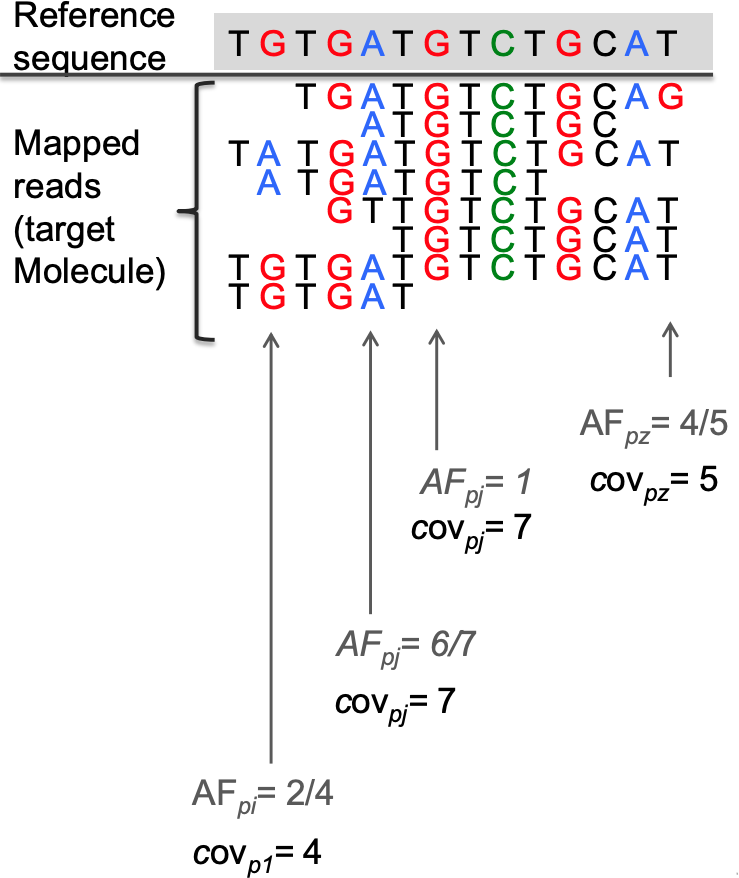
\includegraphics[width=0.4\textwidth]{image14.png}
  \centering
  \caption{View of sequence alignment} \label{fig: coverage and allele
  frequency}
\end{figure}


The \textbf{local coverage} (cov) as shown in figure \ref{fig: coverage and
allele frequency} at position $i$ is the number of reads that span $p_i$.

The \textbf{allelic fraction} (AF) as shown in figure \ref{fig: coverage and
allele frequency} at position $i$ is the proportion of reads that supports the
reference base in $p_i$ (= the reference or the alternative allele).

\subsection{Whole Genome Sequencing Coverage}

\begin{equation} \label{eq: coverage formula}
  cov = \frac{L \dot N}{G}
\end{equation}

where:

\begin{itemize}
\item
  \textbf{L} is the read length.
\item
  \textbf{N} is the number of mapped reads.
\item
  \textbf{G} is the haploid human genome length.
\end{itemize}


This is super important because it saves us time and money when we design an
experiment. When you design an NGS experiment, you should know before what is
the type of coverage you need to answer the question you wanna ask with your
experiment. For example, if you want to look at the genotype of SNPs (inherited
polymorphisms at single side), you don't really need a coverage which is above
$10$ or $15$. So you can design your experiment in order to have an average
coverage equal to $10$ or $15$. To do that, you reverse the equation and count
how many reads you need to generate to achieve that goal. \\

\textit{N.B.}: The number of mapped reads will be always lower of the number of
reads generated by the machine (than the expected). There might be duplicates
that you might not be able to use because there might be reads that have a
quality below the threshold you intend to use.


\hypertarget{difference-between-sequence-coverage-and-physical-coverage}{%
\subsubsection{Difference between sequence coverage and physical
coverage}\label{difference-between-sequence-coverage-and-physical-coverage}}


A graphic view of how \textbf{SE (Single End Sequencing)} or \textbf{PE (Paired
End Sequencing)} can be used:

\begin{figure}[H]
  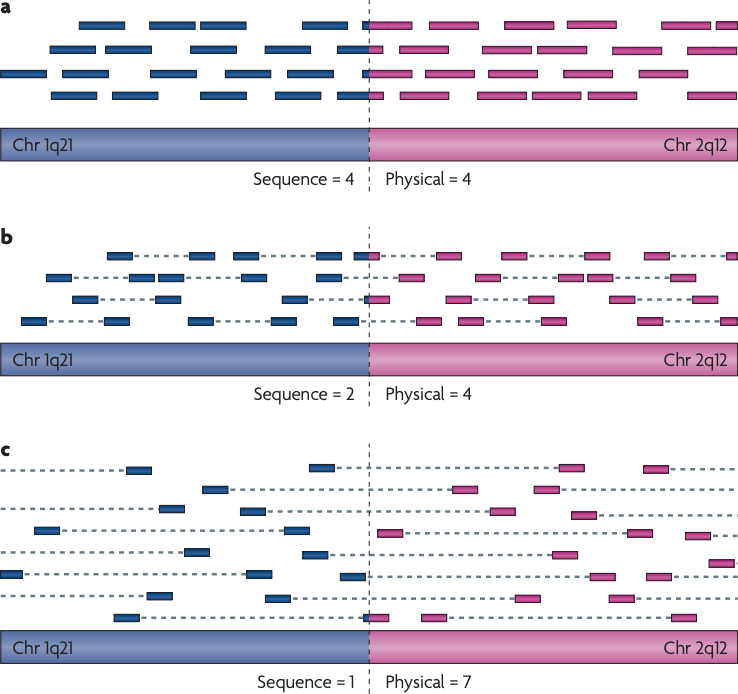
\includegraphics[width=0.65\textwidth]{image15.png}
  \centering
  \caption{Panel A - SE protocol; Panel B - PE protocol; Panel C - PE protocol}
  \label{fig: physical coverage vs coverage}
\end{figure}

Three different scenario are depicted that vary in the length of the DNA
fragments that are sequenced. \textbf{Sequence coverage} represents the number
of sequenced reads that cover the site; this affects the ability to detect point
mutations. \textbf{Physical coverage} measures the number of fragments that span
the site; this affects the ability to detect the rearrangements, based on paired
reads that map to different chromosomes. It is a way informative type of
coverage: for instance for translocations, deletions $\dots$

In Paired End sequencing protocols, the physical coverage is always higher than
the sequence coverage. Choosing the method illustrated in panel 3 (figure
\ref{fig: physical coverage vs coverage}).

Making estimation of intended coverage and observed coverage is very important.
Below I will report an example:\\


\noindent \underline{\textbf{Example coverage observation:}}\\

In these panels were designed to sequence a set of $10$ genes that the
researchers were interested in for prostate cancer. They designed this panel,
sequenced cell lines on this panel and observed the following points

\begin{itemize}
  \item On $x$-axis: the genomic location
  \item On $y$-axis: the local coverage (amplicon median coverage = each bar
  represents the local coverage of about 30 bp)
\end{itemize}

The different colors represent the different genes


\begin{itemize}
  \item \textbf{$1^{st}$ panel}: Local coverage (pile-up) of selected areas
  (targeted sequencing assay): 7 genes

  \begin{itemize}
    \item + 1 multi-gene region (T2ERG). Alternate colors indicate targeted
    areas The barplot show a single sample (LnCaP cell line; cancer cell line)
    data.
    \item Apparent \textbf{deletion} of PTEN (monoallelic deletion) because the
    local coverage of PTEN is significantly lower than the one from other genes.
  \end{itemize}
  
  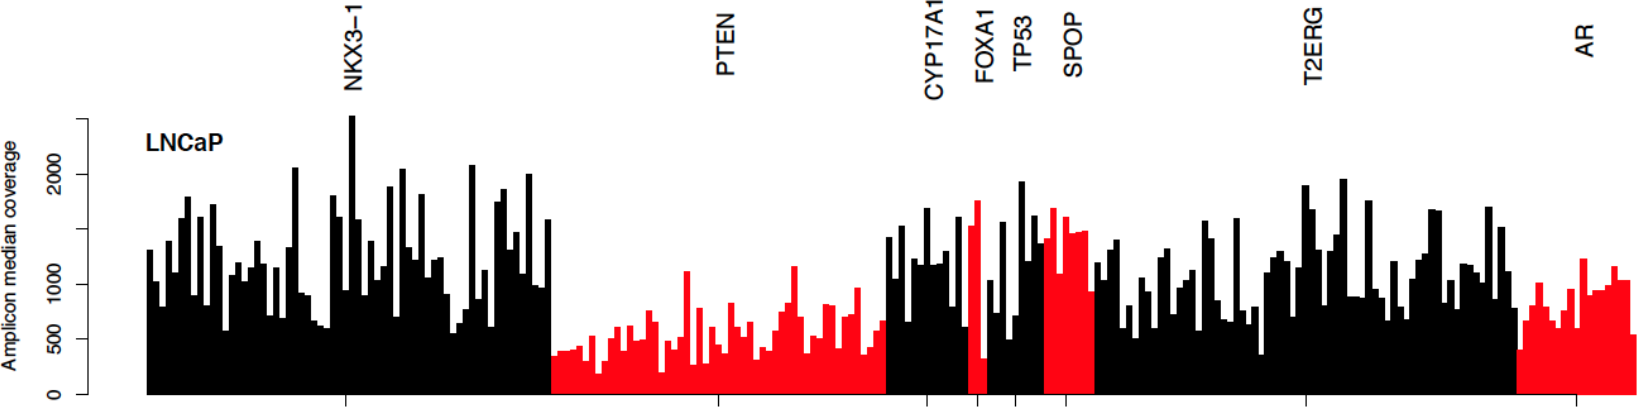
\includegraphics[width=6.13481in,height=1.52625in]{image16.png}

  \item \textbf{$2^{nd}$ panel}: Local coverage (pile-up) of selected areas
  (targeted sequencing assay): 7 genes

  \begin{itemize}
    \item + 1 multi-gene region.
    \item Monoallelic deletion and partial biallelic deletion of PTEN because
    one portion is deleted and one not. PTEN has a \textbf{partial homozygous
    deletion}.
    \item The PC3 cell line shows a little bit of gain in the gene SPOP and
    FOXA1.
    \item The average coverage for the PC3 cells is approximately the same as
    the previous sample.
  \end{itemize}
  
  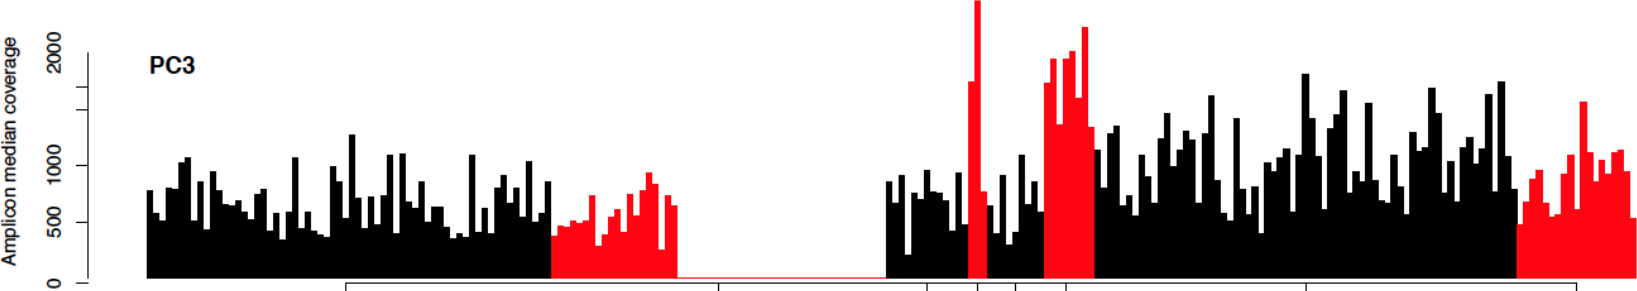
\includegraphics[width=6.15327in,height=1.09125in]{image17.png}

  \item \textbf{$3$rd panel}: 
  
  \begin{itemize}
    \item There's no homozygous deletion but has a high level
    \textbf{amplification} of one area \emph{absorbs} all the reads. Massive
    amplification of the Androgen Receptor (AR) → error: because it inhibits the
    sensitivity of detecting copy number changes in any other gene, the signal
    is excessively intense.
    \item When designing a panel we must pay attention and make sure that we
    don't have potential aberration that basically will draw all the attention
    of your experiment and leave you without information or \textbf{sensitivity}
    in all other regions.
    \item  It's easy to \underline{increase the experimental coverage (i.e. the
    sequence depth) at later point}. Provided tour original sample/library is
    still available, you can perform another run of sequencing and then combine
    the output from different runs.
  \end{itemize}

  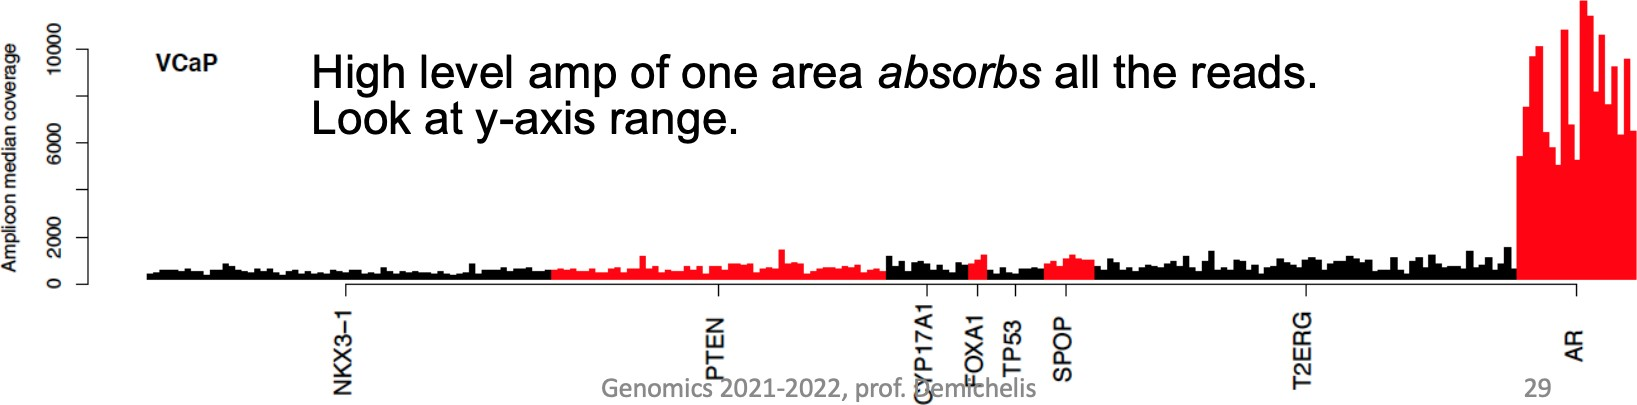
\includegraphics[width=6.17134in,height=1.51875in]{image18.jpeg}
\end{itemize}


\hypertarget{note-that-this-isnt-possible-with-array-based-technologies.}{%
\subsubsection{Note that this isn't possible with array-based
technologies.}\label{note-that-this-isnt-possible-with-array-based-technologies.}}


What are the limiting factors of NGS DNA-seq experiment, in any?

Repeated regions due to \textbf{short reads}

What is the problem of short sequencing on long genome?

\begin{itemize}
  \item Complexity regions
  \item GC content
\end{itemize}
% #TODO non ho capito questo commento 


\hypertarget{the-reference-sequence-of-the-human-genome}{%
\section{The reference sequence of the human
genome}\label{the-reference-sequence-of-the-human-genome}}


Many years ago, some people claimed that the entire human genome was sequenced
but it wasn't true at all. There were still unknown or missing regions. In 2022
we finally have the complete human reference genome sequence.

But we need to consider the polymorphisms, there is no \textbf{unique} genome.
How to integrate them into a single reference genome? There is a consortium that
deals with these problems. They assemble a reference genome that reflects the
most common (in the whole population) sequences at each position of the human
genome, but also tracks information of everything that is polymorphic. So that
we can use the latest release of what they built as reference genome and then
use databases to learn about all the polymorphic sites and all the features of
every polymorphic variants.

Genome Reference Consortium:
(\href{https://www.ncbi.nlm.nih.gov/grc/human}{Genome Reference Consortium
link}) where you can find different versions of human reference genome

UCSC Genome Browser on Human: (\href{http://genome-euro.ucsc.edu/}{UCSC link})

where you can upload different versions of the reference


\hypertarget{interpreting-pair-orientation}{%
\subsection{Interpreting pair orientation}\label{interpreting-pair-orientation}}


Using IGV (Integrative Genomics Viewer) (see chapter \ref{chap: IGV} for more
details)

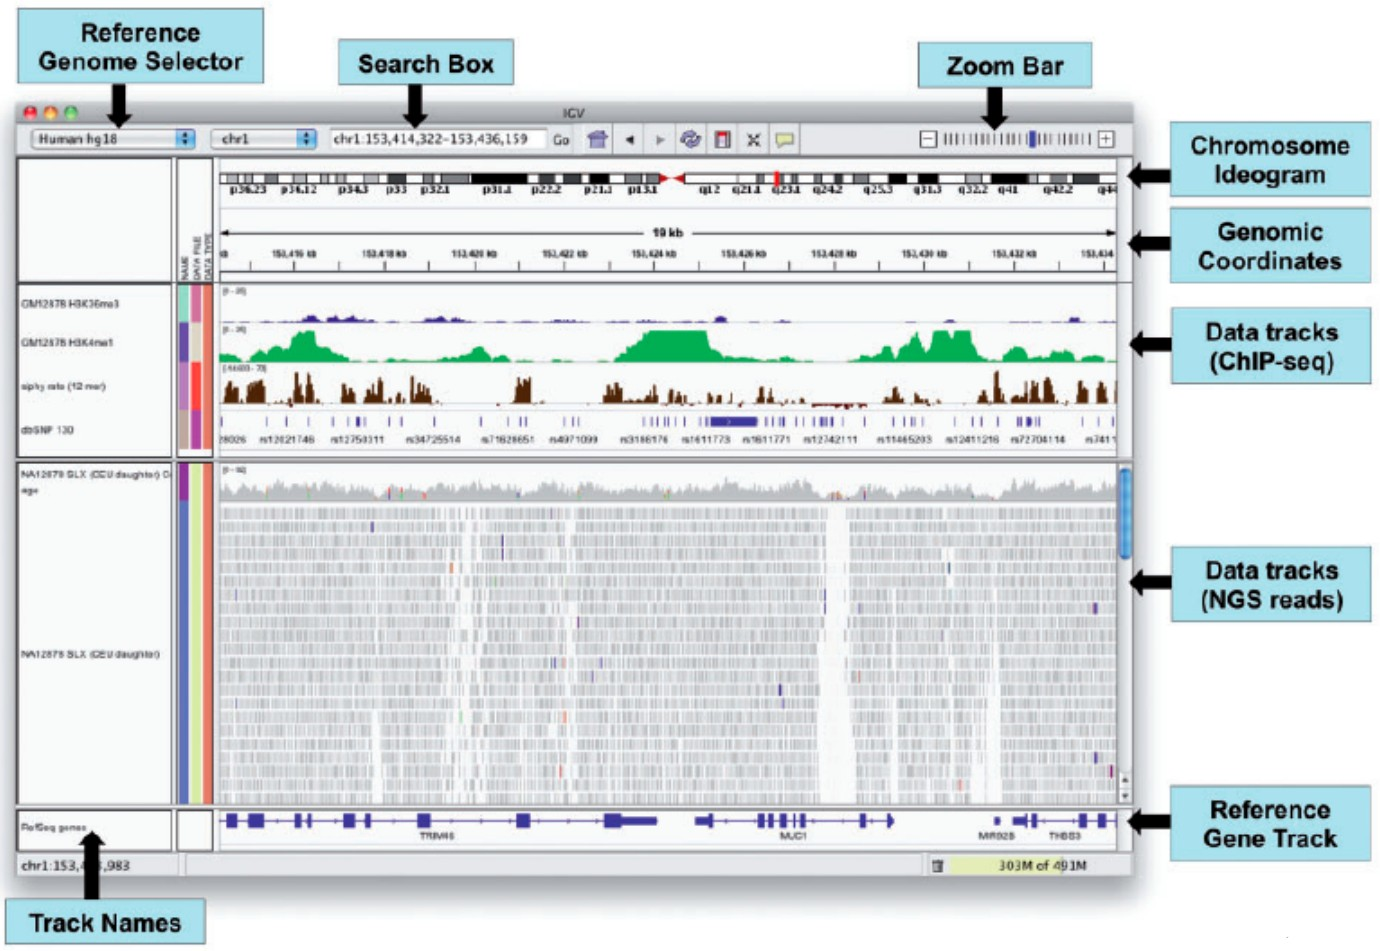
\includegraphics[width=6.32631in,height=4.35875in]{image19.jpeg}

The main characteristic of IGV is that it is a main view viewer: all the
information are in one window.

On the x-axis there's the genome coordinates at the top, the reference genome at
the bottom (we can select the reference genome we prefer).

Along with the data tracks there is the local coverage of the kb shown in the
window (of the sample we are looking at).

You can get any information you want of any single read that you are uploading,
very useful to see difference from the reference genome because every aberration
or whatsoever is highlighted by a different color in the local coverage of a
nucleotide base. Moreover, it gives information about the quality of the read
and the bases, if you have a PE protocol, it tells you also information about
the PE for each of them.

The \textbf{orientation} of paired end can be used to detect structural events,
including: 

\begin{itemize}
  \item Inversions
  \item Duplications
  \item Translocations
\end{itemize}


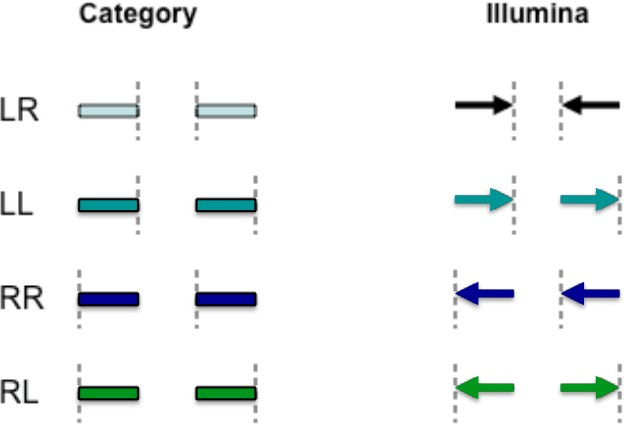
\includegraphics[width=3.89062in,height=2.65in]{image20.jpeg}


\hypertarget{inversion}{%
\subsection{Inversion}\label{inversion}}


A segment of DNA is inverted\\


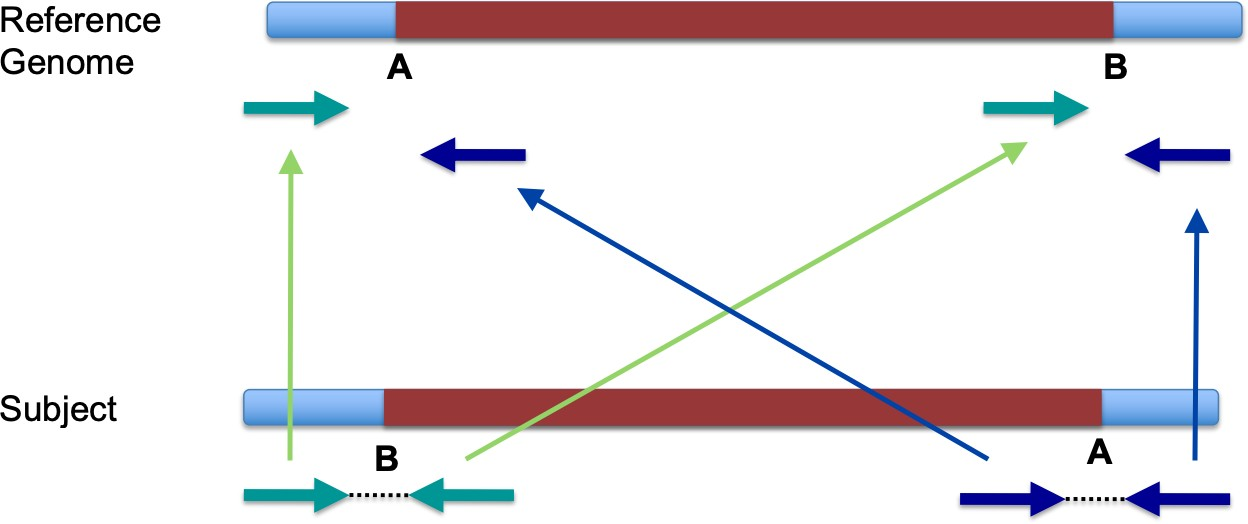
\includegraphics[width=5.85745in,height=2.45625in]{image21.jpeg}


The most important pairs are the ones that stand between junctions because they
are the most informative ones.

Here one end mapped where it was on the reference genome while the other end
reversed its orientation.\\

In IGV:\\


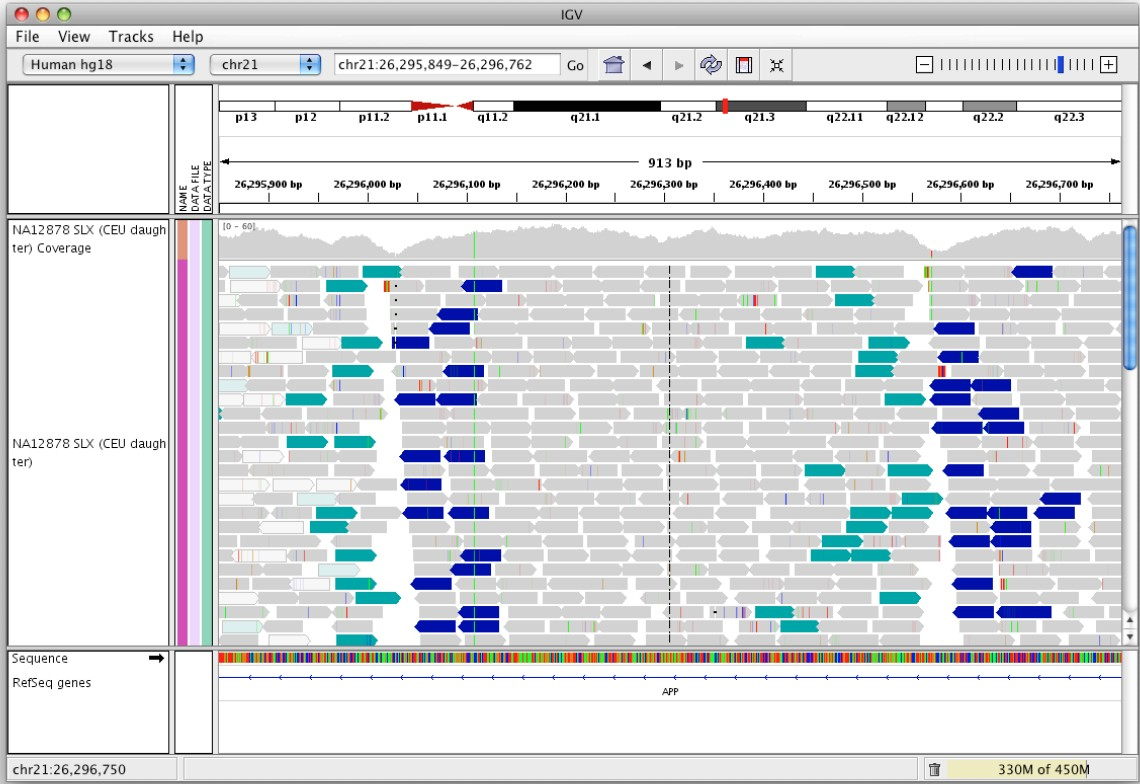
\includegraphics[width=6.29861in,height=4.32833in]{image22.jpeg}


Information that help us:

\begin{itemize}
  \item The \textbf{insert size} from the target molecule (= the subject) is way
  longer. For all the pairs that are at the breakpoint, the insert size is
  different from the expected.

  \item The \textbf{orientation} is different.
  
  \item If you look at the local coverage, you can see a \textbf{drop} in two
  points: at the breakpoints. The reads that are mapping the junctions cannot
  map the reference genome because the breakpoint sequence is altereed in the
  reference genome. So, if we have an inversion in only one of the two alleles,
  then the reads coming from the allele with the inversion will not contribute
  to the local coverage at the breakpoint. The contribution to the local
  coverage will come only from one allele.
\end{itemize}


Moreover, we can notice that the coverage on the middle part does not change
significantly from the coverage on the sides.

When you align reads against a genome, you can \underline{allow for a certain
mismatches or partial alignment}. So, if you impose certain thresholds to your
aligner, you can also say that if there are reads that align for 80\% and have
20\% of sequences misaligned, you align them in any case. So you will have reads
that are correct up to the breakpoints and the browser will shows the mismatches
beyond the breakpoint. So, you can have a partial drop of coverage because you
allow mismatches in your alignment.


\hypertarget{tandem-duplication}{%
\subsection{Tandem duplication}\label{tandem-duplication}}


A segment of DNA is duplicated and inserted in the target molecule adjacent to
the original one.


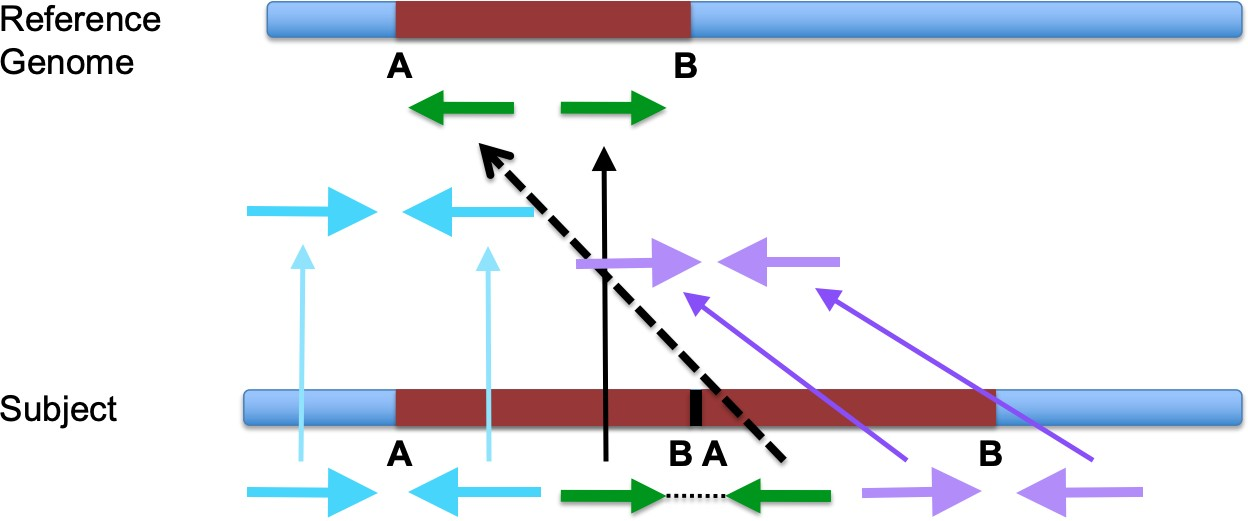
\includegraphics[width=6.1113in,height=2.55073in]{image23.jpeg}\\

So, as result, the orientation instead of going inward goes outward.\\

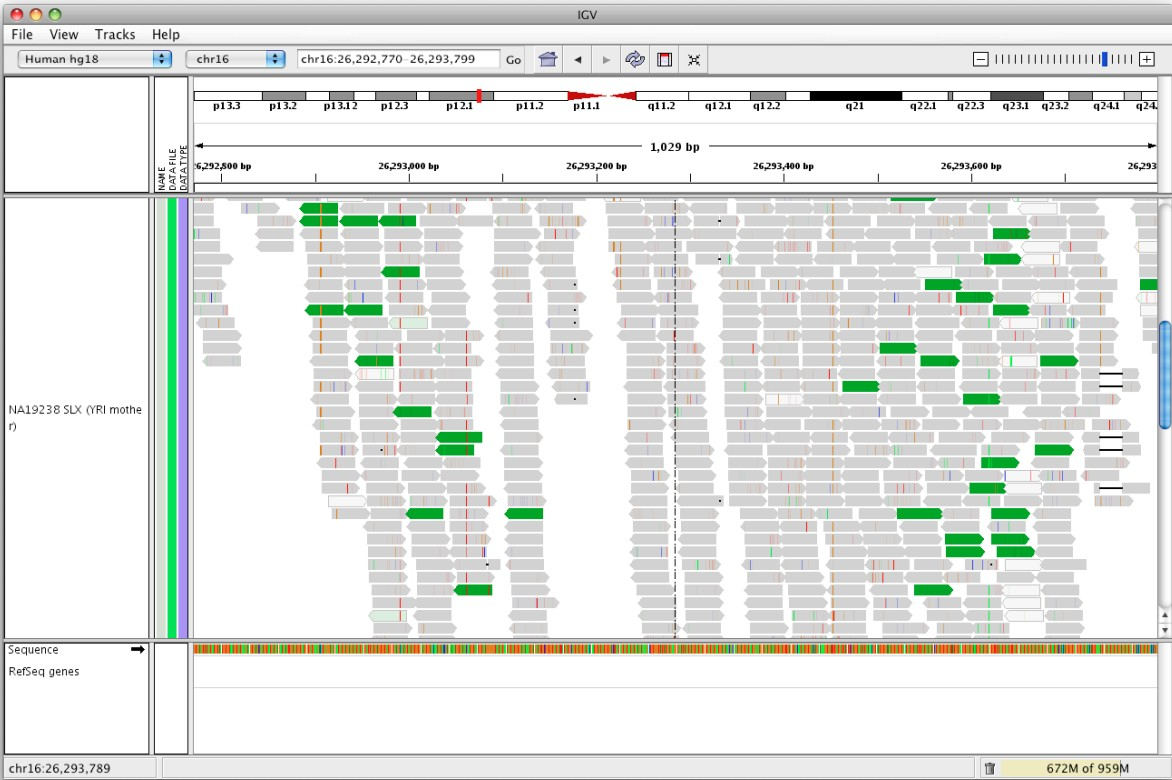
\includegraphics[width=6.22598in,height=4.14375in]{image24.jpeg}\\

\emph{What do you expect to see from coverage?} We will have a gain in coverage
that is proportional to the extra copy. We need to pay attention to the double
because it is a double contribution of that allele, but if a tandem duplication
happens only in one allele and the other allele has his own one copy, then the
local coverage corresponding to the tandem duplication will be 3/2 of the
expected coverage.\\

If you have a read that maps BA, do you expect to see it in the mapped reads?
Partial mapping. As we said before, if you allow your mapper to have some
mismatches of a certain percentage of bases from your reads, you can still see
some coverage contributed on one end of the segment and mismatches on the other
side.
% #TODO da riscrivere

For what concern the \underline{junctions}, you shouldn't see any difference of
coverage because that sequence exists only once in the target molecule. The
local coverage increases only in correspondence of the segment AB.


\hypertarget{inverted-duplication}{%
\subsection{Inverted duplication}\label{inverted-duplication}}


The duplication is inverted but it's not located near the original fragment, but
somewhere else.

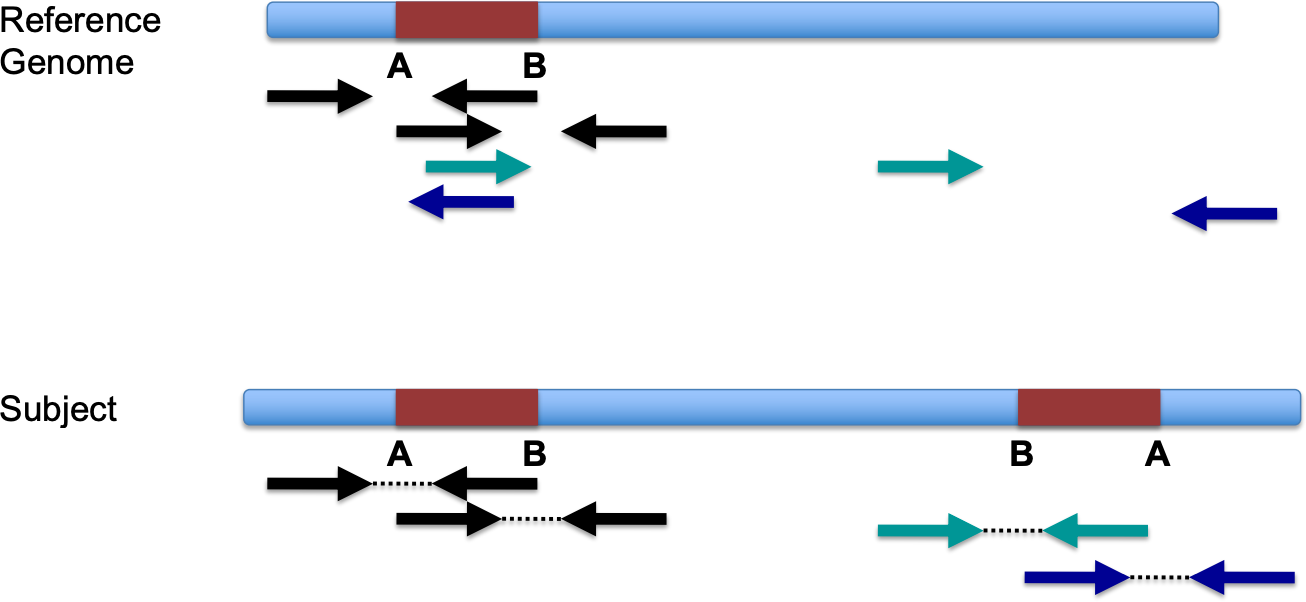
\includegraphics[width=6.11483in,height=2.82187in]{image25.png}\\


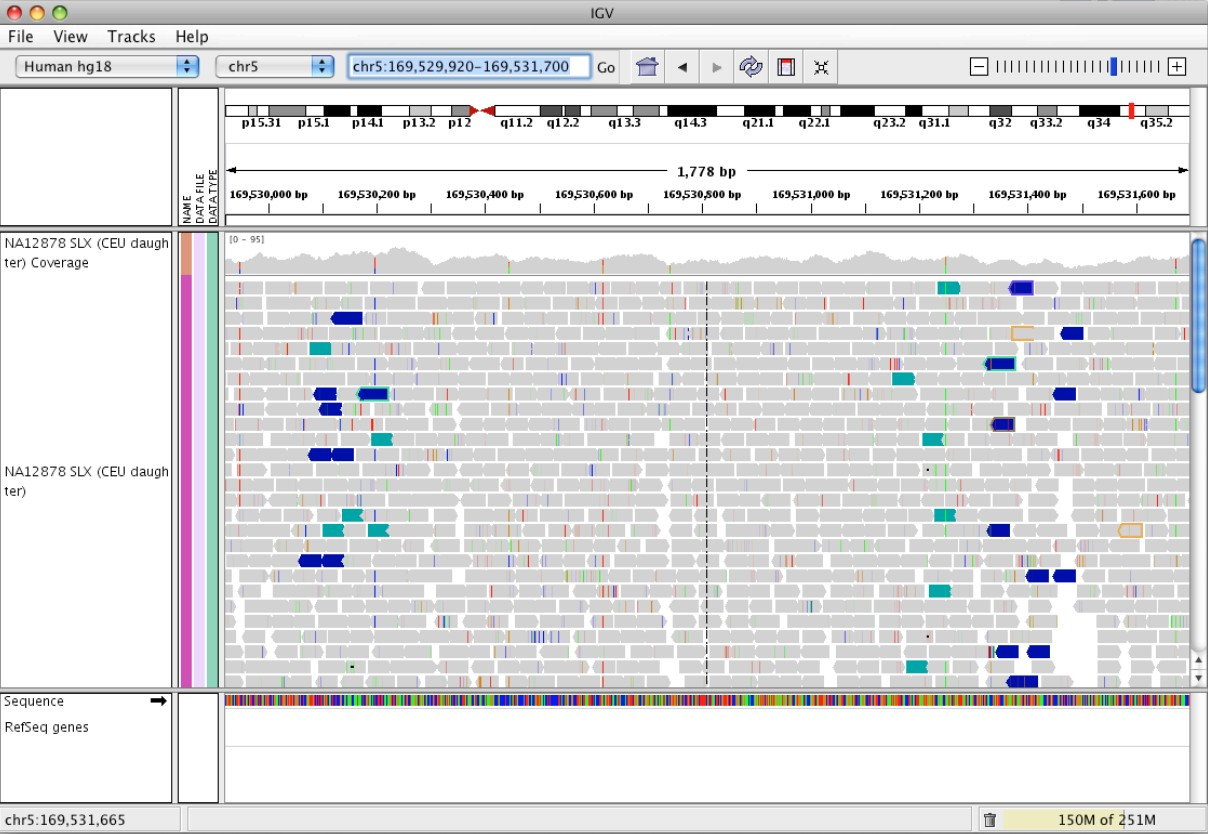
\includegraphics[width=6.29059in,height=4.34375in]{image26.jpeg}\\


There is a gain of coverage in the duplicated region and a tiny drop in the
break points where the sequence exists in only one allele.


\hypertarget{deletion}{%
\subsection{Deletion}\label{deletion}}


Deletion of a segment of DNA:

\begin{itemize}
  \item If the deletion \underline{is larger} than the size of the reads, we
  should see half of the coverage in the deleted regions.
  \item If the deletion \underline{is shorter} that the size of the reads, we
  should see a tiny little space corresponding to the missing nucleotides.

\end{itemize}



